\Needspace{8\baselineskip}\originalchapter{2003 年 MHD 综合期末：椭圆柱的竖直模}
22.615 Spring 2003 历史 take-home final 题卷将原编号1—5作为同一 $n=0$ 竖直位移问题的五步；配有 11 页官方解答，末五页是椭圆坐标附表而非新题。这里按一道综合题、五个原步骤呈现，显式标出独立复算与官方答案一致处。题目用大纵横比 $a/R_0\to0$、零压力 $p\to0$ 及常电流近似判断理想导电壁距；有限电阻壁增长、反馈控制只作物理动机，并非本卷的求解条件。
\begin{exercise}\label{ex:hist03-mhd-1}
原步骤1。实心等离子体截面 $x^2/a^2+y^2/(\kappa^2a^2)=1$，$\kappa>1$；$J_z=-J_0$ 常数，$\nabla^2\psi=-\mu_0R_0J_z=\mu_0R_0J_0$，$\mathbf B_p=R_0^{-1}\nabla\psi\times\hat z$，边界 $\psi=0$。求 $\psi,B_x,B_y$，忽略 $O[(a/R_0)^2]$ 的其余场分量。
\end{exercise}
\begin{solution}
编者独立解答；与官方扫描原步骤1的函数形状、系数一致。设 $\psi=\psi_a[x^2/a^2+y^2/(\kappa^2a^2)-1]$，其 Laplace 值为 $2\psi_a(1+\kappa^{-2})/a^2$，所以
\begin{equation}\psi_a=\frac{\mu_0R_0J_0a^2\kappa^2}{2(1+\kappa^2)},\quad B_x=\frac{2\psi_a y}{R_0\kappa^2a^2},\quad B_y=-\frac{2\psi_a x}{R_0a^2}.\end{equation}
只求内部平衡；外部真空扰动在后续步骤求。边界 $\psi=0$ 不表示扰动 $A$ 也为零。
\end{solution}

\begin{exercise}\label{ex:hist03-mhd-2}
原步骤2。用均匀刚体竖直试位移 $\boldsymbol\xi=\xi_0\hat y$ 计算流体势能 $\delta W_F$，验证它为负。压力为零，且题目规定只保留主阶极向场贡献。
\end{exercise}
\begin{solution}
编者独立解答。$\nabla\cdot\boldsymbol\xi=0$，冻结条件给 $\mathbf B_1=\nabla\times(\boldsymbol\xi\times\mathbf B_p)=-\xi_0\partial_y\mathbf B_p=-2\psi_a\xi_0\hat x/(R_0\kappa^2a^2)$。用主阶理想 MHD 能量式 $\delta W_F=\frac12\int_{V_p}[B_1^2/\mu_0-\boldsymbol\xi\cdot(\mathbf J\times\mathbf B_1)]\dd V$，$\mathbf J=-J_0\hat z$，截面积 $\pi\kappa a^2$、环向长 $2\pi R_0$，得
\begin{equation}\delta W_F=-\frac{4\pi^2\psi_a^2\xi_0^2}{\mu_0R_0a^2\kappa}=-W_0<0,\quad W_0>0.\end{equation}
这个负值说明无壁时试位移能降低流体能；有壁时还必须加真空场正能。公式与官方步骤2核对，不能单独将 $\delta W_F<0$ 宣告有壁系统不稳定。
\end{solution}

\begin{exercise}\label{ex:hist03-mhd-3}
原步骤3。真空扰动写 $\mathbf B_1^v=\nabla A(x,y)\times\hat z$。给真空方程及能量积分；引入共焦坐标 $x=c\sinh u\cos v,y=c\cosh u\sin v$，等离子体 $u=u_1$，理想壁 $u=u_2$，壁竖直高度与等离子体之比 $w=\kappa_wb/(\kappa a)$。用 $a,\kappa,w$ 给出 $c,u_1,u_2,b,\kappa_w$，写壁法向场为零和界面冻结条件，并求 $A(u_1,v)=K\sin v$ 中 $K$。
\end{exercise}
\begin{solution}
编者独立解答。真空无电流令 $\nabla^2A=0$、$\delta W_V=(2\mu_0)^{-1}\int_{V_v}|\nabla A|^2\dd V$。共焦距 $c=a\sqrt{\kappa^2-1}$，$\sinh u_1=1/\sqrt{\kappa^2-1}$、$\cosh u_1=\kappa/\sqrt{\kappa^2-1}$；$\cosh u_2=w\kappa/\sqrt{\kappa^2-1}$，故
\begin{equation}b=a\sqrt{w^2\kappa^2-\kappa^2+1},\quad
\kappa_w=\frac{w\kappa}{\sqrt{w^2\kappa^2-\kappa^2+1}},\quad
u_2=\operatorname{arcosh}\!\frac{w\kappa}{\sqrt{\kappa^2-1}}.\end{equation}
上式最后的 $u_2$ 是椭圆径向坐标（不是角 $v$）。壁 $\hat n\cdot\mathbf B_1^v=0$ 等价 $\partial_v A(u_2,v)=0$；把壁上常数规范设 $A(u_2,v)=0$。界面 $\hat n\cdot\mathbf B_1^v=\hat n\cdot\nabla\times(\boldsymbol\xi\times\mathbf B_p)$，代步骤1的 $B_x$ 和几何度规，积分 $v$ 后得 $A(u_1,v)=K\sin v$，
\begin{equation}K=-\frac{2\psi_a\xi_0}{R_0a\kappa}.
\end{equation}
与官方步骤3一致。共焦要求 $w>1$；当 $\kappa\to1$ 时椭圆坐标退化，但最终圆极限可由连续极限取得。
\end{solution}

\begin{exercise}\label{ex:hist03-mhd-4}
原步骤4。在步骤3的共焦真空环域解 $A$ 并计算 $\delta W_V$，保留壁间距 $u_2-u_1$ 依赖。
\end{exercise}
\begin{solution}
编者独立解答。椭圆坐标共形，$\nabla^2A=h^{-2}(\partial_u^2+\partial_v^2)A$；单一 $\sin v$ 谐波使径向方程 $F''-F=0$。两边界值给
\begin{equation}A(u,v)=K\,\frac{\sinh(u_2-u)}{\sinh(u_2-u_1)}\sin v.
\end{equation}
用 Green 第一恒等式，$\nabla^2A=0$ 时体积分 $\int|\nabla A|^2$ 化为内边界 $-\int A\partial_uA\dd v$ 乘 $2\pi R_0$；$\int_0^{2\pi}\sin^2v\dd v=\pi$，故
\begin{equation}\delta W_V=\frac{4\pi^2\psi_a^2\xi_0^2}{\mu_0R_0a^2\kappa^2}\coth(u_2-u_1)>0.
\end{equation}
壁越近，$\coth(u_2-u_1)$ 越大，真空压缩场更难，符合导电壁稳定化的物理预期，也与官方步骤4核对。
\end{solution}

\begin{exercise}\label{ex:hist03-mhd-5}
原步骤5。合并 $\delta W_F,\delta W_V$，令边际稳定 $\delta W=0$，求最小壁高比 $w=w(\kappa)$ 并作曲线；说明 $\kappa\to1,\infty$ 与 $\kappa=2$ 的数值。
\end{exercise}
\begin{solution}
编者独立解答。令 $C=4\pi^2\psi_a^2\xi_0^2/(\mu_0R_0a^2\kappa^2)>0$，则 $\delta W=C[\coth(u_2-u_1)-\kappa]$。边际式 $\coth(u_2-u_1)=\kappa$。由 $\tanh u_1=1/\kappa$、$\tanh u_2=1/\kappa_w$，代双曲差公式，得边际壁纵横比 $\kappa_w=(\kappa^2+1)/(2\kappa)$，再代步骤3的共焦关系，化简为
\begin{equation}\boxed{w_{\rm crit}(\kappa)=\frac{\kappa^2+1}{\kappa\sqrt{\kappa^2-1}}},\qquad\kappa>1.
\end{equation}
固定 $\kappa$ 时 $w<w_{\rm crit}$（壁更近）给 $\delta W>0$，所试竖直模稳定；$w>w_{\rm crit}$ 给负能。$\kappa\downarrow1$ 时临界比趋无穷（圆截面无同样的竖直伸长驱动），$\kappa\to\infty$ 时趋1；$\kappa=2$ 给 $5/(2\sqrt3)\simeq1.443$。与官方步骤5式和极限一致。下图为公式直接绘制，不是对扫描图描摹：
\begin{center}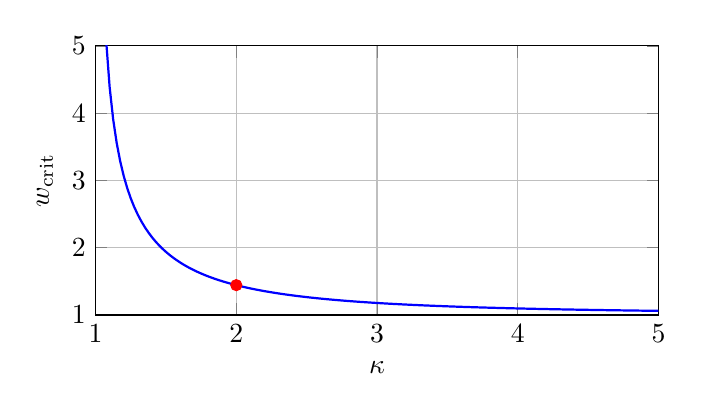
\begin{tikzpicture}\begin{axis}[width=.72\textwidth,height=5cm,xlabel={$\kappa$},ylabel={$w_{\rm crit}$},xmin=1,xmax=5,ymin=1,ymax=5,grid=both,samples=160,domain=1.025:5]\addplot[blue,thick]{(x^2+1)/(x*sqrt(x^2-1))};\addplot[only marks,mark=*,red] coordinates {(2,1.443375673)};\end{axis}\end{tikzpicture}\end{center}
能量法使用特定刚体试函数；负 $\delta W$ 足以示不稳定，正值只表示该试函数未找到负能，不能单凭此称所有可能位移皆稳定。官方解答在本近似模型内把其边际曲线作为目标结果。
\end{solution}
